\newpage
\section{Umsetzung (ca. 10 Seiten)}
\label{Umsetzung}
Nachdem die theoretischen Grundlagen im letzten Kapitel vorgestellt wurden, wird in diesem Kapitel die Umsetzung beschrieben. Dieses Kapitel wird nach einem geordneten Vorgehen strukturiert. Zuerst werden verfügbare Daten vorgestellt, analysiert und sortiert. In diesem Schritt wird entschieden, welche Daten die Zielvariable Nachfrage beeinflussen und somit mit in das Modell eingegeben werden. Die deskriptive Analyse unterstützt dabei die Visualisierung der Daten und verleiht mehr Verständnis für den zeitlichen Einsatz und die Verteilung der Kosten innerhalb der Medienkanäle. Darauffolgend werden die Daten in das \ac{OLS}-Modell eingesetzt. Die Ergebnisse des Modells werden analysiert.

\subsection{Einsatz der deskriptiven Analyse für die Datenbewertung}
Wie im Kapitel \nameref{deskriptiveanalyse} beschrieben, fasst die deskriptive Analyse historische Daten zusammen und zeigt wichtige Muster und Trends auf. Sie bildet die Grundlage für weiterführende Analysen und datengestützte Entscheidungen. Um auf den Einsatz des \ac{OLS}-Modells vorzubereiten, werden die Daten vom \ac{MMM} deskriptiv analysiert. \\\\
Für das \ac{MMM}-Modell (s. \autoref{fig:mmmbonprix}) stehen Daten vom 01.01.2022 bis 01.01.2024 zur Verfügung. Diese Daten umfassen die Marketing-Ausgaben, wie Katalogausgaben, Online-Marketingausgaben und Mediaausgaben. Für Mediakanäle sind spezifisch auch die Kosten der Unterkanäle dabei. 
Unter diesen Daten fallen auch Kosten für (adressierbares) TV, Podcasts, \ac{dooh}+\ac{ooh}, Radio, YouTube, soziale Medien, Online-Videos und Display-Medien. Für die internen Faktoren sind Kosten von E-Mail, Push-Nachrichten und Verkaufsförderungen wie Versandkostenbefreiung und Rabatt verfügbar. Für die externen Faktoren ist ein Saisonalitätswert von einem Facebook-Saisonmodell vorhanden. Um die Wettbewerber im Modell zu berücksichtigen, sind auch Marketingausgaben von C\&A, H\&M, About You und Zalando verfügbar. Zum Schluss ermöglichen Nachfrage und Datum, den Verlauf sowie die Auswirkungen aller Faktoren auf Tagesbasis darzustellen. \\\\
Da es auf der Media-Ebene modelliert wird, werden nicht alle Daten von dem \ac{MMM} benötigt. Für den Anfang werden nur für Media relevante Daten für das Modell entnommen. Die Daten werden von der Google BigQuery Cloud in die Google Jupyter-Notebook-Instanz geladen, um dort mit Python modelliert zu werden. Die Daten bilden eine Tabelle, in der jede Zeile nach Datum sortiert ist und einen Tag mit den Informationen aller Variablen darstellt. \\\\
Zuerst wird die Qualität der Daten für das \ac{MMM} überprüft. Wie im \autoref{methodederkleinstenquadrate} beschrieben, führen Redundanzen zu einem falschen Ergebnis im Modell. Deshalb soll es überprüft werden, ob es allgemein Redundanzen in den Zeilen gibt. Auch ohne \(y_i\) kann der Koeffizient $\beta$ nicht geschätzt werden. In dem Media-Modell ist die Nachfrage der Zielwert \(y_i\), da es gerechnet werden soll, wie viel ein Euro als Ausgabe in einem Media-Kanal in der Nachfrage bringt. Die Nachfrage darf deswegen nicht Null sein. Daher wird im ersten Schritt überprüft, ob allgemein Redundanzen vorliegen und ob in der Spalte \anf{demand} Nullwerte vorhanden sind.\\\\
So wurde der Code \verb|df_raw[df_raw['demand'].isnull()]| ausgeführt, um Zeilen mit einem leeren Nachfrage-Wert abzufragen. Dabei wurde eine Zeile mit einem leeren Nachfrage-Wert am 29.06.2024 identifiziert. Um den Null-Wert zu korrigieren, wurde der Durchschnitt der Nachfragen am 28.06.2024 und am 30.06.2024 für das Datum 29.06.2024 berechnet und eingesetzt.  
\begin{lstlisting}[language=Python, linewidth=\textwidth]
mask = (df_raw['date'] == '2024-06-29')
avg_demand = df_raw.loc[df_raw['date'].isin(['2024-06-28', '2024-06-30']), 'demand'].mean()
df_raw.loc[mask, 'demand'] = avg_demand
\end{lstlisting}
Nach der Datenverarbeitung wurde ein Überblick über den Datenverlauf geschaffen, um die erste Forschungsfrage in \nameref{ZielsetzungDerArbeit}
zu beantworten. Es wurde untersucht, wie sich die Mediaausgaben verhalten und welche möglichen Auswirkungen sie auf die Nachfrage haben. Mithilfe des Codes im \nameref{Anhang1:ZeitlicherVerlaufMitPywidgets} wird ein Liniendiagramm erstellt, bei dem die x-Achse die Zeit auf Tagesbasis darstellt. Die linke y-Achse zeigt die prozentualen Werte für die Ausgaben der Media-Kanäle, während die rechte y-Achse die prozentualen Werte für die Nachfrage darstellt. Um die Visualisierung flexibel zu gestalten, wird mithilfe von \verb|ipywidgets| eine interaktive Datendarstellung mit Auswahllisten erstellt. Diese Auswahllisten ermöglichen es, zwischen verschiedenen Media-Kanälen zu wechseln und ein flexibles Startdatum zwischen dem 01.01.2022 und dem 01.01.2025 für die x-Achse im Diagramm auszuwählen. Die prozentualen Werte der y-Achsen werden berechnet, indem die Tagesausgaben durch die Gesamtausgaben dividiert werden. Die Berechnung der prozentualen Werte ermöglicht einen besseren Vergleich zwischen den beiden Werten und vermeidet eine Darstellung mit absoluten Zahlen. Diese Ausgaben werden nach der Auswahl eines Datums neu berechnet, um eine zeitgemäße Darstellung zu gewährleisten. \\\\
Das Kapitel \nameref{MediaKanäleInDerPraxis} beschreibt, dass Generali eine gute Erfahrung mit YouTube als Media-Kanal hat. Auch die Metaanalyse von Nielsen besagt, dass YouTube beim \ac{ROI} das TV übertrifft. Also wird der YouTube-Verlauf mit dem Verlauf der Nachfrage zuerst verglichen:\\\\
\begin{figure}[ht]
    \centering
    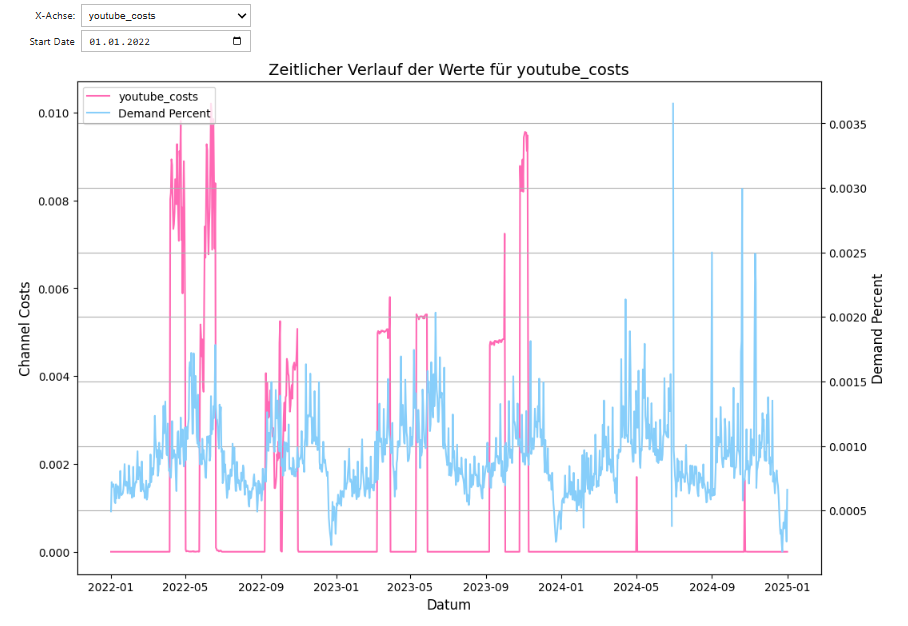
\includegraphics[width=0.98\linewidth]{images/youtubeLineChart.png}
    \caption{Liniendiagramm: Ein Vergleich von YouTube-Ausgaben und Nachfrage, eigene Darstellung}
    \label{fig:youtubelinechart-label}
\end{figure}
Aus dem Liniendiagramm in \autoref{fig:youtubelinechart-label} geht hervor, dass die YouTube-Ausgaben sporadisch auftreten. Wie im \autoref{MediaKanäleBeiBonprix} beschrieben, entstehen Ausgaben für diesen Media-Kanal in einem begrenzten Zeitraum, etwa für einen Monat. Auch hier ist es zu erkennen, dass für den Kanal YouTube zweimal Kosten anfallen, mit einem kurzen zeitlichen Abstand. Die YouTube-Ausgaben treten meist um Mai und kurz nach September auf. Dies ist auch der Zeitraum, in dem die Nachfrage etwas höher ist. \\\\
Mit bloßem Auge ist nicht erkennbar, ob ein Zusammenhang zwischen den Mediaausgaben und der Nachfrage besteht. Allerdings ähnelt der Verlauf der Online-Marketingausgaben dem Verlauf der Nachfrage. Im Liniendiagramm in \autoref{fig:omaverlauf} ist zu erkennen, dass der Verlauf von Online-Marketing und Nachfrage nahezu übereinstimmt. Das weist daraufhin, dass das Online-Marketing möglicherweise einen großen Einfluss auf die Nachfrage hat und im Modell zu berücksichtigen ist.
\begin{figure}[H]
    \centering
    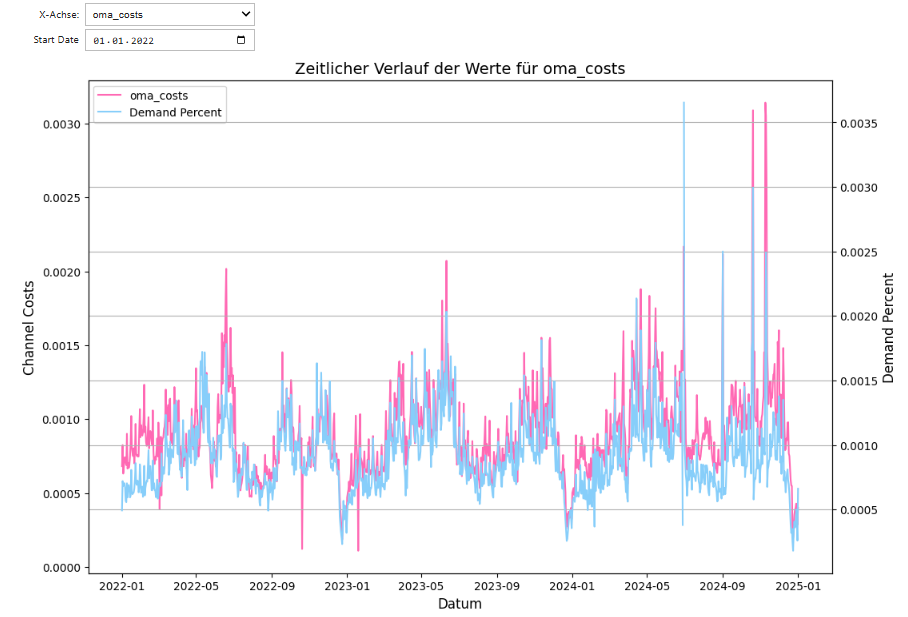
\includegraphics[width=0.8\linewidth]{images/omacosts.png}
    \caption{Verlauf von Ausgaben des Online-Marketings und Nachfrage ab 01.01.2022, eigene Darstellung}
    \label{fig:omaverlauf}
\end{figure}
Neben dem Online-Marketing hat auch die Verkaufsförderung einen möglichen Einfluss auf die Nachfrage. In \autoref{fig:verlaufvonverkaufsförderung} ist zu erkennen, dass zwischen Juli 2024 und Dezember 2024 vier hohe Spitzen der Nachfrage und Verkaufsförderungskosten parallel entstanden sind. 
\begin{figure}[H]
    \centering
    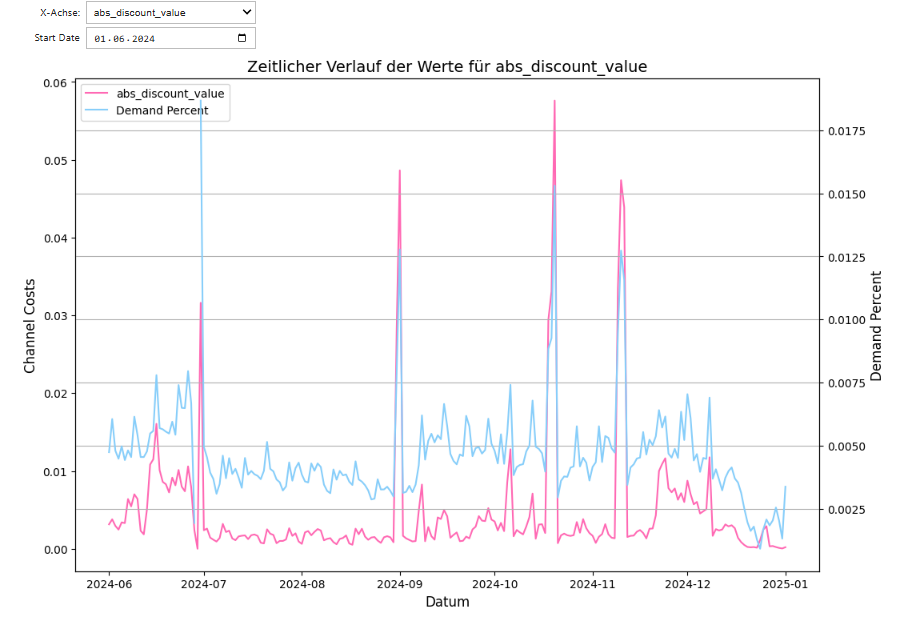
\includegraphics[width=0.8\linewidth]{images/vf_sum.png}
    \caption{Verlauf von Verkaufsförderung und Nachfrage ab 01.06.2024, eigene Darstellung}
    \label{fig:verlaufvonverkaufsförderung}
\end{figure}
Es wird erwartet, dass Einflussfaktoren wie Online-Marketing und Verkaufsförderung einen sofortigen Einfluss auf die Nachfrage haben. Eine Erhöhung der Ausgaben für solche Faktoren führt zu einem sofortigen Anstieg der Nachfrage. Im Vergleich dazu haben Medienkanäle wie YouTube keinen direkt erkennbaren Effekt auf die Nachfrage. Es wird angenommen, dass der Effekt von Media-Kanäle milder und nachhaltiger auf das Konsumverhalten ist. Um den Nachfrageeffekt von Media-Kanäle zu quantifizieren, wird später die Huber-Regression eingesetzt und der \ac{ROAS} berechnet.
\begin{figure}[H]
    \centering
    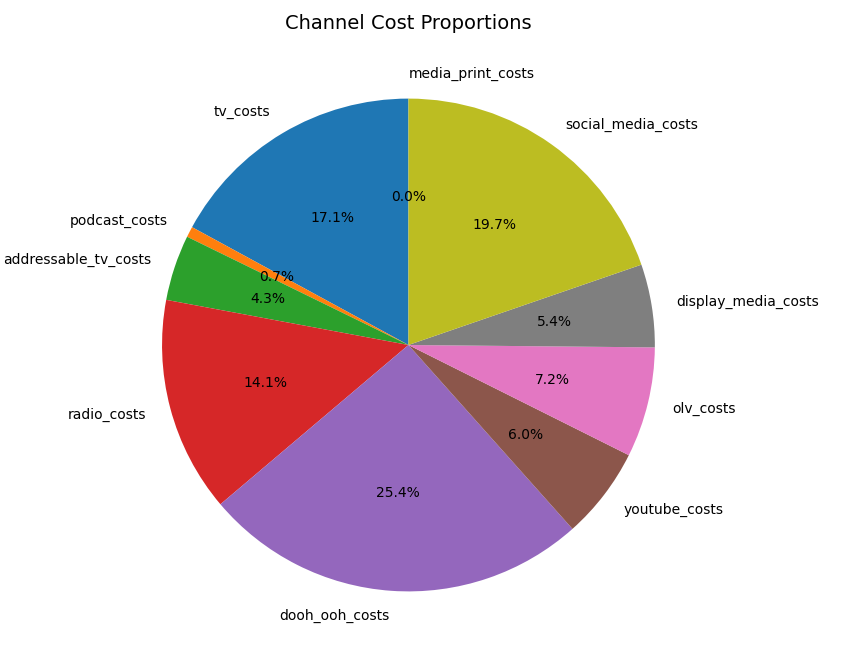
\includegraphics[width=0.8\linewidth]{images/mediapie.png}
    \caption{Kostenanteil der Media-Kanäle bei bonprix, eigene Darstellung}
    \label{fig:mediapie}
\end{figure}
Um die Verteilung der Ausgaben für Media-Kanäle besser zu verstehen, werden die Ausgabenanteile der Media-Kanäle in einem Kreisdiagramm visualisiert. Der Code im \nameref{Anhang2KreisdiagrammAufteilungDerMediaausgaben} ermöglicht ebenfalls die Interaktion mit dem Startdatum und erstellt das Kreisdiagramm in \autoref{fig:mediapie} mit einem Startdatum von 01.01.2022.\\\\
% ROI
In diesem Kreisdiagramm in \autoref{fig:mediapie} ist es zu erkennen, dass die YouTube-Ausgaben einen relativ kleinen Anteil von 6\% betragen. Das entspricht etwas mehr als einem Drittel der TV-Ausgaben, die 17,1 \% betragen. Wenn \nameref{MediaKanäleInDerPraxis} zutrifft, dass YouTube mehr \ac{ROI} als TV erbringt und wenn die Trainingsdaten vollständig sind, wird erwartet, dass YouTube einen höheren \ac{ROAS} als TV aufweist. Es wird erwartet, dass in der optimalen Aufteilung YouTube einen höheren Anteil als in der Gegenwart aufweist. Die höchsten Kosten entfallen auf die Kombination von \ac{dooh} und \ac{ooh}, die einen Anteil von 25,4 \% aufweist.
\newpage
\subsection{Prüfung und Umgang mit Multikollinearität}
\label{PrüfungUndUmgangMitMultikollinearität}
Wie im \autoref{einschränkungenderregression} beschrieben, muss die Kollinearität zwischen den Prädiktoren behoben werden. Als Erstes wird die Korrelationsmatrix der Prädiktoren untersucht. Mithilfe der Methode \verb|.corr()| wird die Korrelation zwischen den Prädiktoren berechnet. Anschließend wird die Korrelation mit der Funktion \verb|.heatmap| aus der Bibliothek \verb|seaborn| farblich visualisiert.
\begin{figure}[H]
    \centering
    \begin{lstlisting}[language=Python, linewidth=\textwidth]
df_corr_media=dfcmedia.corr() 
plt.figure(figsize=(15, 12))
sns.heatmap(df_corr_media, annot=True, cmap='coolwarm', fmt=".2f")
plt.title("Korrelationsmatrix")
plt.show()
\end{lstlisting}
    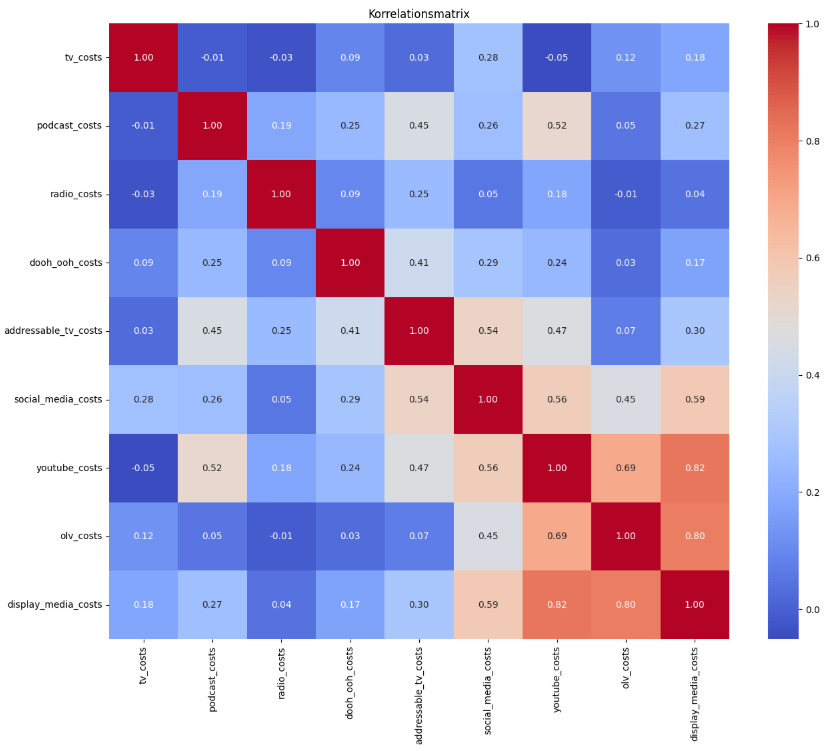
\includegraphics[width=1\linewidth]{images/korrelationsmatrix.png}
    \caption{Korrelationsmatrix der Prädiktoren, eigene Darstellung}
    \label{fig:korrelationsmatrix}
\end{figure}
Wie im \autoref{einschränkungenderregression} beschrieben, weist ein großer absoluter Wert in der Korrelationsmatrix auf eine hohe Korrelation hin. Das bedeutet, dass sowohl Werte nahe -1 als auch nahe 1 eine hohe Korrelation beschreiben. Die negative Korrelation ist unproblematisch, da der Betrag der negativen Werte alle gleich oder unter 0,05 bleibt. Hingegen ist die positive Korrelation problematisch. Paare wie YouTube mit Display Media, \ac{olv} mit Display Media, YouTube mit \ac{olv}, YouTube mit Social Media, Social Media mit Display Media haben alle einen Wert von mindestens 0,56. \\\\
Es wird mit einer Untersuchung von \ac{VIF} fortgesetzt. Zuerst werden numerische Werte herausgefiltert. Danach werden Werte ohne Veränderung, also Standardabweichung gleich 0, mit \verb|.std() > 0| entfernt. Zum Schluss wird mithilfe der Methode \verb|variance_inflation_factor()| der \ac{VIF} ausgerechnet. 
\begin{lstlisting}[language=Python, linewidth=\textwidth][H]
X = X.select_dtypes(include=[np.number]) 
X = X.loc[:, X.std() > 0]
vif = pd.DataFrame()
vif["Variable"] = X.columns
vif["VIF"] = [variance_inflation_factor(X.values, i) for i in range(X.shape[1])]
print(vif)
\end{lstlisting}
\begin{table}[h]
    \centering
    \begin{tabular}{@{}ll@{}}
        \toprule
        Variable               & VIF       \\ \midrule
        tv\_costs              & 1.376725  \\
        podcast\_costs         & 1.946688  \\
        addressable\_tv\_costs & 2.257337  \\
        radio\_costs           & 1.143652  \\
        dooh\_ooh\_costs       & 1.321926  \\
        youtube\_costs         & 7.717482  \\
        olv\_costs             & 4.336781  \\
        display\_media\_costs  & 6.224349  \\
        social\_media\_costs   & 2.658416  \\ \bottomrule
    \end{tabular}
    \label{tab:viftabelle}
    \caption{Variance Inflation Factor (VIF) for Variables, eigene Darstellung}
\end{table}
In der \hyperref[tab:viftabelle]{Tabelle VIF} wird erkannt, dass YouTube und Display Media jeweils einen \ac{VIF}-Wert über 5 besitzen. Nach \autoref{einschränkungenderregression} werden sie als problematisch eingestuft. Basierend auf den Erfahrungen in der Abteilung wird ein \ac{VIF}-Wert ab 2 als problematisch angesehen. \ac{olv}, Social Media und eventuell adressierbarer TV werden daher als problematisch betrachtet. Dies bestätigt auch die hohen Korrelationswerte in der \autoref{fig:korrelationsmatrix}. Nach dem Austausch mit der Media-Abteilung wird bestätigt, dass Display Media, YouTube, \ac{olv} und Social Media oft zusammen aktiviert werden. In der Analyse werden diese Kanäle deshalb als Variable \verb|video_costs| zusammengefasst: 
\begin{lstlisting}
df["video_costs"] = df["youtube_costs"] + df["olv_costs"] + 
                df["display_media_costs"] + df["social_media_costs"]
\end{lstlisting}
Nach der Verarbeitung von den Prädiktoren wird die hohe Korrelation in der Korrelationsmatrix in \autoref{fig:korrelationsmatrix-danach} beseitigt.
\begin{figure}
    \centering
    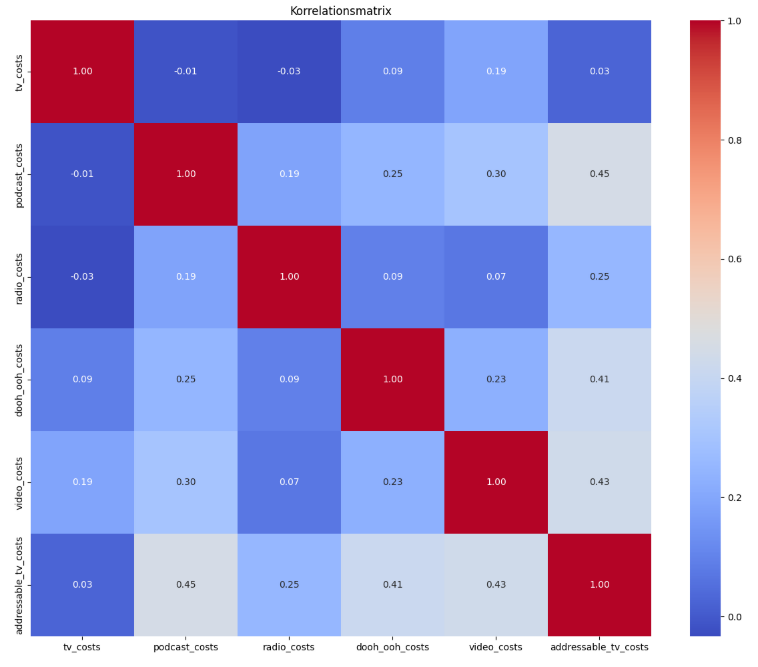
\includegraphics[width=1\linewidth]{images/korrelationafter.png}
    \caption{Korrelationsmatrix nach der Behebung von hoher Korrelation, eigene Darstellung}
    \label{fig:korrelationsmatrix-danach}
\end{figure}
\subsection{Einsatz des Marketing-Mix-Modells}
\begin{figure}
    \centering
    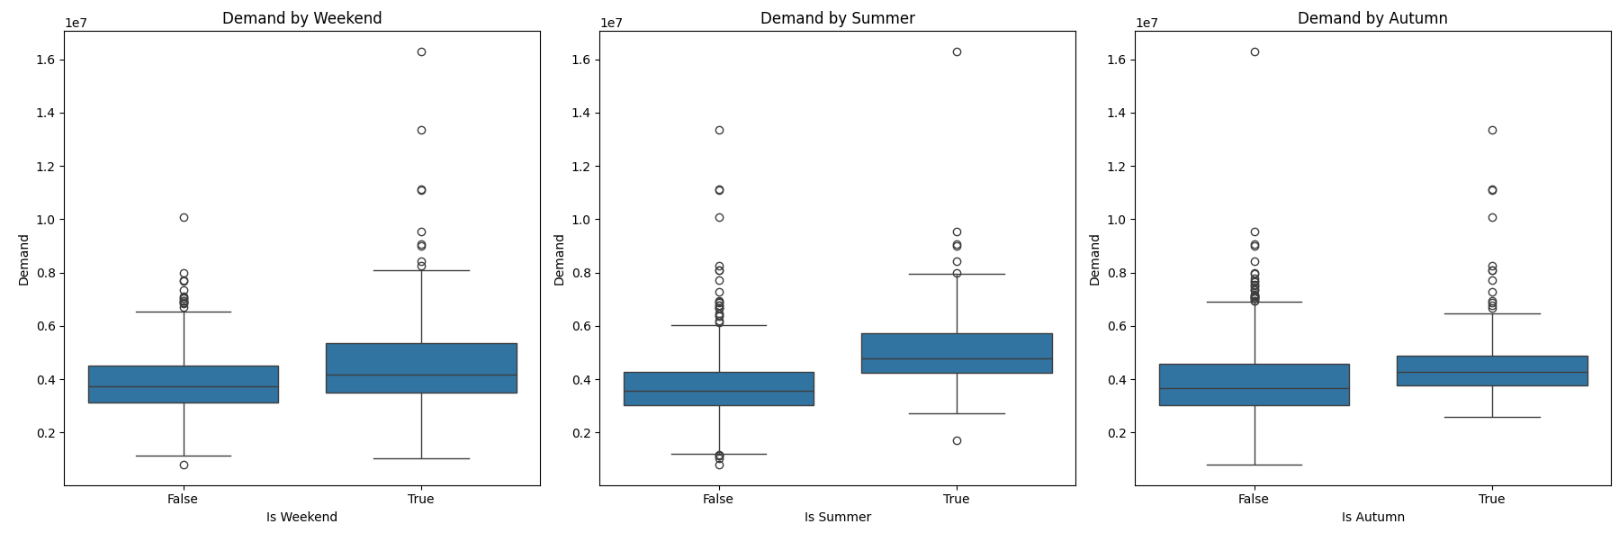
\includegraphics[width=1\linewidth]{images/boxplot.png}
    \caption{Boxplot: Nachfrage-Streuung mit Saisonalität, eigene Darstellung}
    \label{fig:boxplotsaison}
\end{figure}
